\documentclass[conference]{IEEEtran}
\makeatletter
\def\ps@headings{%
\def\@oddhead{\mbox{}\scriptsize\rightmark \hfil \thepage}%
\def\@evenhead{\scriptsize\thepage \hfil \leftmark\mbox{}}%
\def\@oddfoot{}%
\def\@evenfoot{}}
\makeatother
\pagestyle{headings}

\newcommand{\thetitle}{On the Linear Structure of Network Traffic: Predicting Flow Behavior}

%!TEX root = paper.tex

\usepackage[labelfont=bf,small]{caption}
\usepackage[font=small,labelfont=bf,position=top,nearskip=0em]{subfig}
\usepackage{cite,amsmath,amssymb,rotating,multirow,bigstrut,url,wrapfig,relsize,paralist,array,mathtools,units}
\usepackage[hyperfigures,bookmarks,bookmarksopen,bookmarksnumbered,colorlinks,linkcolor=black,citecolor=black,filecolor=blue,menucolor=black,pagecolor=blue,frenchlinks=true,pdftitle={\thetitle}]{hyperref}

%!TEX root = paper.tex

%% LABELING COMMANDS
\renewcommand{\sec}[1]{\label{sec:#1}}
\newcommand{\eqn}[1]{\label{eqn:#1}}
\newcommand{\fig}[1]{\label{fig:#1}}
\newcommand{\tab}[1]{\label{tab:#1}}
\newcommand{\thm}[1]{\label{thm:#1}}
\newcommand{\defn}[1]{\label{def:#1}}

%% REFERENCING COMMANDS
\newcommand{\Appendix}[1]{\hyperref[sec:#1]{Appendix~\ref*{sec:#1}}}
\newcommand{\Section}[1]{\hyperref[sec:#1]{Section~\ref*{sec:#1}}}
\newcommand{\Equation}[1]{\hyperref[eqn:#1]{Equation~\ref*{eqn:#1}}}
\newcommand{\Figure}[1]{\hyperref[fig:#1]{Figure~\ref*{fig:#1}}}
\newcommand{\Table}[1]{\hyperref[tab:#1]{Table~\ref*{tab:#1}}}
\newcommand{\Theorem}[1]{\hyperref[thm:#1]{Theorem~\ref*{thm:#1}}}
\newcommand{\Definition}[1]{\hyperref[def:#1]{Definition~\ref*{def:#1}}}

%% MATHEMATICAL NOTATIONS

% common algebraic domains
\newcommand{\N}{\mathbb{N}}
\newcommand{\Z}{\mathbb{Z}}
\newcommand{\Q}{\mathbb{Q}}
\newcommand{\R}{\mathbb{R}}

% standard operators & functors
\renewcommand{\Pr}{\mathrm{Pr}}
\newcommand{\Image}{\text{Im}}
\newcommand{\Kernel}{\text{Ker}}

% common constructs
\newcommand{\abs}[1]{{\left|#1\right|}}
\newcommand{\absx}[1]{{|#1|}}
\newcommand{\card}[1]{{\left|#1\right|}}
\newcommand{\cardx}[1]{{|#1|}}
\newcommand{\norm}[1]{{\lVert#1\rVert}}
\newcommand{\normx}[1]{{\Vert#1\Vert}}
\newcommand{\set}[1]{{\left\{#1\right\}}}
\newcommand{\setx}[1]{{\{#1\}}}
\newcommand{\parens}[1]{{\left(#1\right)}}
\newcommand{\parensx}[1]{{(#1)}}
\newcommand{\bracket}[1]{{\left[#1\right]}}
\newcommand{\bracketx}[1]{{[#1]}}
\newcommand{\seq}[1]{{\left<#1\right>}}
\newcommand{\seqx}[1]{{\lvert#1\rvert}}
\newcommand{\tuple}[1]{{\left<#1\right>}}
\newcommand{\tuplex}[1]{{\lvert#1\rvert}}
\newcommand{\floor}[1]{{\left\lfloor#1\right\rfloor}}
\newcommand{\floorx}[1]{{\lfloor#1\rfloor}}
\newcommand{\ceil}[1]{{\left\lceil#1\right\rceil}}
\newcommand{\ceilx}[1]{{\lceil#1\rceil}}
\newcommand{\round}[1]{{\left[#1\right]}}
\newcommand{\roundx}[1]{{[#1]}}
\newcommand{\fracx}[2]{{#1/#2}}
\newcommand{\fracp}[2]{{\left(\frac{#1}{#2}\right)}}
\newcommand{\fracpx}[2]{{(#1/#2)}}
\newcommand{\smallfrac}[2]{{\textstyle{\frac{#1}{#2}}}}

% standard notations
\newcommand{\trans}[1]{{#1}^T}
\newcommand{\inner}[2]{{#1}\trans{#2}}
\newcommand{\cross}{\times}
\newcommand{\tensor}{\otimes}
\newcommand{\directsum}{\oplus}
\newcommand{\iso}{\cong}
\newcommand{\union}{\cup}
\newcommand{\inter}{\cap}
\newcommand{\disunion}{\sqcup}
\newcommand{\Union}{\bigcup}
\newcommand{\Inter}{\bigcap}
\newcommand{\Disunion}{\bigsqcup}
\newcommand{\conj}{\wedge}
\newcommand{\disj}{\vee}
\newcommand{\Conj}{\bigwedge}
\newcommand{\Disj}{\bigvee}
\newcommand{\defeq}{=}
\renewcommand{\emptyset}{\varnothing}
\renewcommand{\setminus}{\,\raisebox{1pt}{$\smallsetminus$}\,}
\newcommand{\eldiv}{\,./\,}
\newcommand{\diag}{\text{diag}}
\newcommand{\rs}{\text{rs}}
\newcommand{\argmin}{\text{arg min}}

%% FORMATTING BEHAVIORS
\newcommand{\caps}[1]{{\small{#1}}}
\newcommand{\latin}[1]{\textit{#1}}
\newcommand{\defterm}[1]{\textit{#1}}
\newcommand{\newfootnote}[2]{\newcommand{#1}{\footnote{#2} }}
\renewcommand{\bullet}{\raisebox{2pt}{$\centerdot$}}
\renewcommand{\arraystretch}{1.3}

%% MISCELLANEOUS

\renewcommand{\vec}[1]{\mathbf{#1}}


\title{\vspace{-0.25em}\thetitle}
\author{
{\large{Stefan~Karpinski, John~R.~Gilbert, Elizabeth~M.~Belding}} \vspace{0.25em}\\
Department of Computer Science \\
University of California, Santa Barbara \vspace{0.35em}\\
\textit{\{sgk,gilbert,ebelding\}@cs.ucsb.edu}
}

\bibliographystyle{IEEEtran}

\newcommand{\figurename}{Figure}
\newcommand{\tablename}{Table}

\begin{document}
\maketitle

\section{Introduction}\sec{introduction}

\newfootnote{\flownote}{We use the common definition of a \textit{flow} as a sequence of packets sharing the same  ``5-tuple'': IP protocol type, source and destination nodes, and TCP/UDP port numbers.}

This paper is the first in a three-part series, employing non-parametric discrete mixture modeling to understand and analyze network traffic patterns at the level of individual flows and packets.\flownote
All three papers employ the same theoretical framework but investigate different fundamental applications of traffic modeling:
prediction, classification and generation.
In this paper we first present the framework and then demonstrate how it can predict detailed behavior of individual flows from the observation of only a handful of initial packets.
% The following papers will focus on classification of flows according to application type and realistic workload generation.

The fundamental concept underlying this work is \emph{linear representation of network traffic}~\cite{Karpinski08}.
A linear representation is a function that maps sets of flows to vectors, the coordinates of which describe aspects of flow behavior;
it must distribute additively over set unions.
% the representation must also satisfy a simple linearity condition which we will describe in detail later.
% the sum of the representations of a set of flows is a vector that represents the aggregate behavior of the set of flows.
An entire traffic trace may be represented as a matrix whose rows are the representations of flows in the trace.
We restrict our consideration to a particularly natural and powerful class of representations whose coordinates are the frequencies of flow features in a set of flows.
For example, the representation can have a dimension for each packet size up to 1500; coordinates in these dimensions indicate the number of packets of each size.
Port numbers, \caps{IP} protocol type, and inter-packet intervals can be handled similarly.
% Examples of flow features are the number of packets of a certain size or the use of a particular port number.
% The fundamental premise of this work, and of the sequel, is that the representatives of actual flow behaviors can be understood as being sampled from 

The essential observation of this research is that under such representations, real flows tend to lie near a small set of low-rank subspaces.
This property allows us to perform a drastic model reduction on trace traffic patterns while preserving the essential characteristics of the original traffic.
Moreover, when observable characteristics of flows are separated from features to be predicted, this model reduction is similar to a classical linear regression:
it allows us to use a least squares optimization on observed features to predict behavior.
We use this technique to predict the following characteristics of each flow from observing only a handful of its initial packets:
\begin{enumerate}
  \item the distribution of packets sizes,
  \item the distribution of inter-packet intervals,
  \item the number of packets that will be in the flow.
\end{enumerate}
From these properties we can indirectly predict many other properties, including the total duration and data volume.

At this point it may be wise to address what we mean by prediction.
Brief reflection shows that one cannot hope to accurately predict the exact behavior of flows:
flow behavior is nondeterministic---flows may exhibit the same initial behavior but subsequently behave quite differently.
The best we can do then is to predict a \emph{distribution} of possible outcomes given the observed initial behavior.
When compared with a specific outcome, such a prediction cannot be said to be ``wrong'' or ``right.''
How then can one measure the quality of a predicted distribution of outcomes?
This subtle and difficult issue is central to our evaluation methodology.

% real-world network traces tend to have approximately low-rank representation matrices despite the potential rank of such matrices being very large.
% Moreover, most flows' vectors lie on only one of a few even lower rank subspaces.
% Moreover, the low-rank subspace near which real traffic lies can be decomposed into subspaces of even lower rank, with almost all flows lying in one of these subspaces.
% Typically, these smaller subspaces are one-dimensional, but in some cases they may have up to a dozen dimensions.

% the vast majority of observed flow behaviors in any given trace lie in one of a handful low-rank subspaces.
% These subspaces are mostly of rank one, but a few have dimensions as high as ten.

% Karpinski~\emph{et~al.}~\cite{Karpinski08} further observed that the simplifications commonly used in traffic modeling correspond to multiplication of traffic representation matrices by low-rank matrices, averaging over rows or columns.
% They demonstrated experimentally that such simplifications severely distort important behavioral properties of traffic traces;
% viewing these simplification as low-rank matrix transformations, this is unsurprising:
% most of the detail of the original traffic behavior is destroyed.
% It was suggested that matrix factorization provides an alternative and superior means of model reduction.

\section{Background \& Motivation}\sec{background}\sec{motivation}

The most fundamental tool for investigating linear structure in high dimensions is the singular value decomposition (\caps{SVD}).
This matrix decomposition can be applied to any real matrix and factors it into a product of three real matrices:
\begin{align}
  X = US\trans{V}.
\end{align}
Here $U$ and $V$ are orthogonal and $S$ is diagonal, with entries of decreasing nonnegative value.
Among the useful properties of this factorization, if all but the first $k$ diagonal entries of $S$ are zeroed out, the product $US_k\trans{V}$ is the best rank-$k$ approximation of $X$ under the Frobenius matrix norm.
The rows of $US_k$ can thus be viewed as an optimal $k$-dimensional reduced model of the rows of $X$, with a new coordinate system given by the columns of $V$.

We can visualize the $k$-dimensional approximate structure of $X$ in $k$ dimensions using the coordinates of $US_k$.
However, the most significant feature of any vector in this representation is its magnitude.
We are more interested in the direction vectors than their direction:
points with the same direction lie in the same one-dimensional subspace.
To visualize direction while eliminating distance, we project all data points radially onto the hyperplane in which all points have coordinates summing to unity.\footnote{We could normalize the vectors to unit length, but then our projection would be spherical, artificially introducing curvature into our visualization.}
% Then we simply scatter-plot various pairs of dimensions of the resulting data.
\Figure{svd} shows scatter plots of the most significant two projected \caps{SVD} coordinates for four different traces.
The original coordinates of this data encode the packet size distributions, inter-packet interval distributions, \caps{IP} protocol numbers, and port numbers for a sample of 5000 flows for each trace.
The exact details of how the linear representation encodes these features will be discussed in \Section{methodology}.

\begin{figure}[!t]
\vspace{0.5em}
\begin{center}
\subfloat[\footnotesize{IETF 60}]{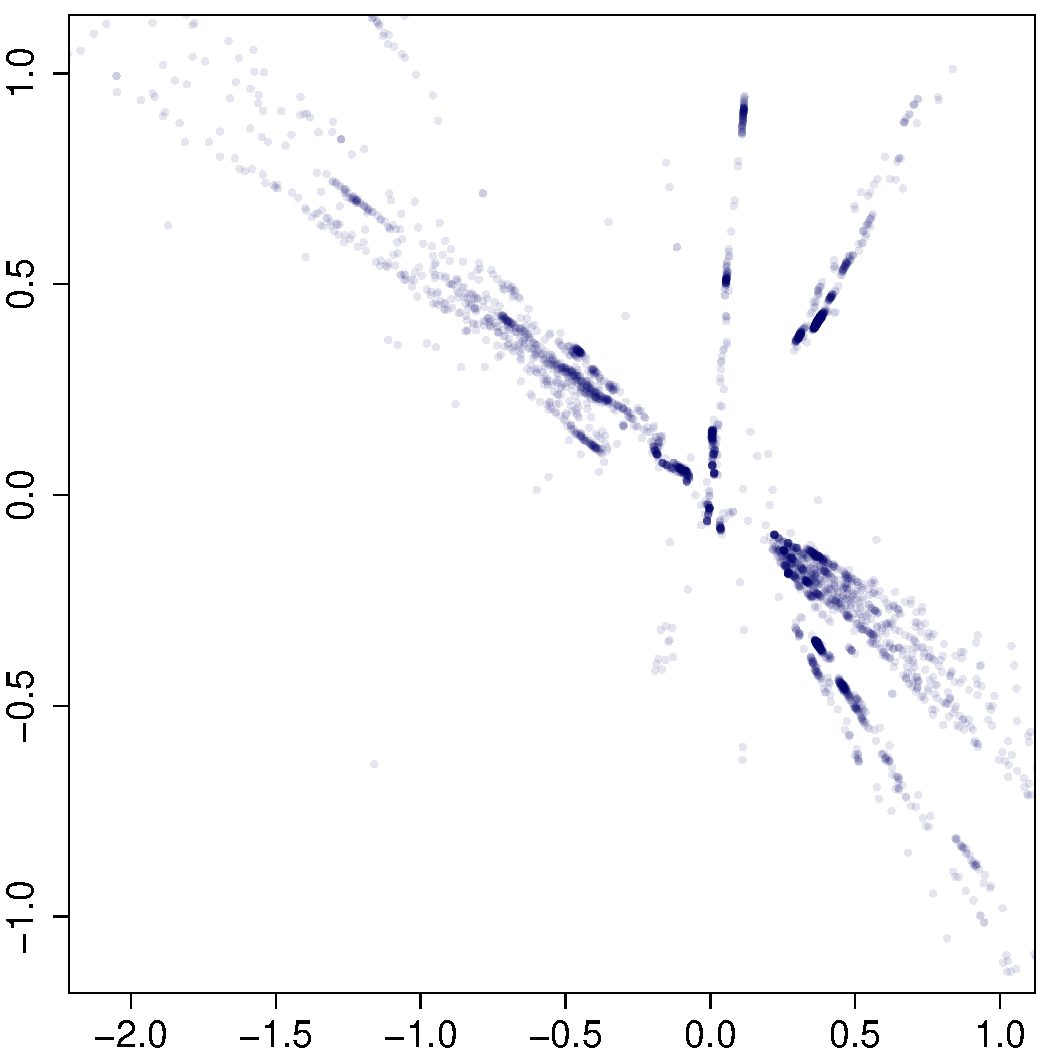
\includegraphics[width=1.6in]{svd/ie60}}
\subfloat[\footnotesize{IETF 67}]{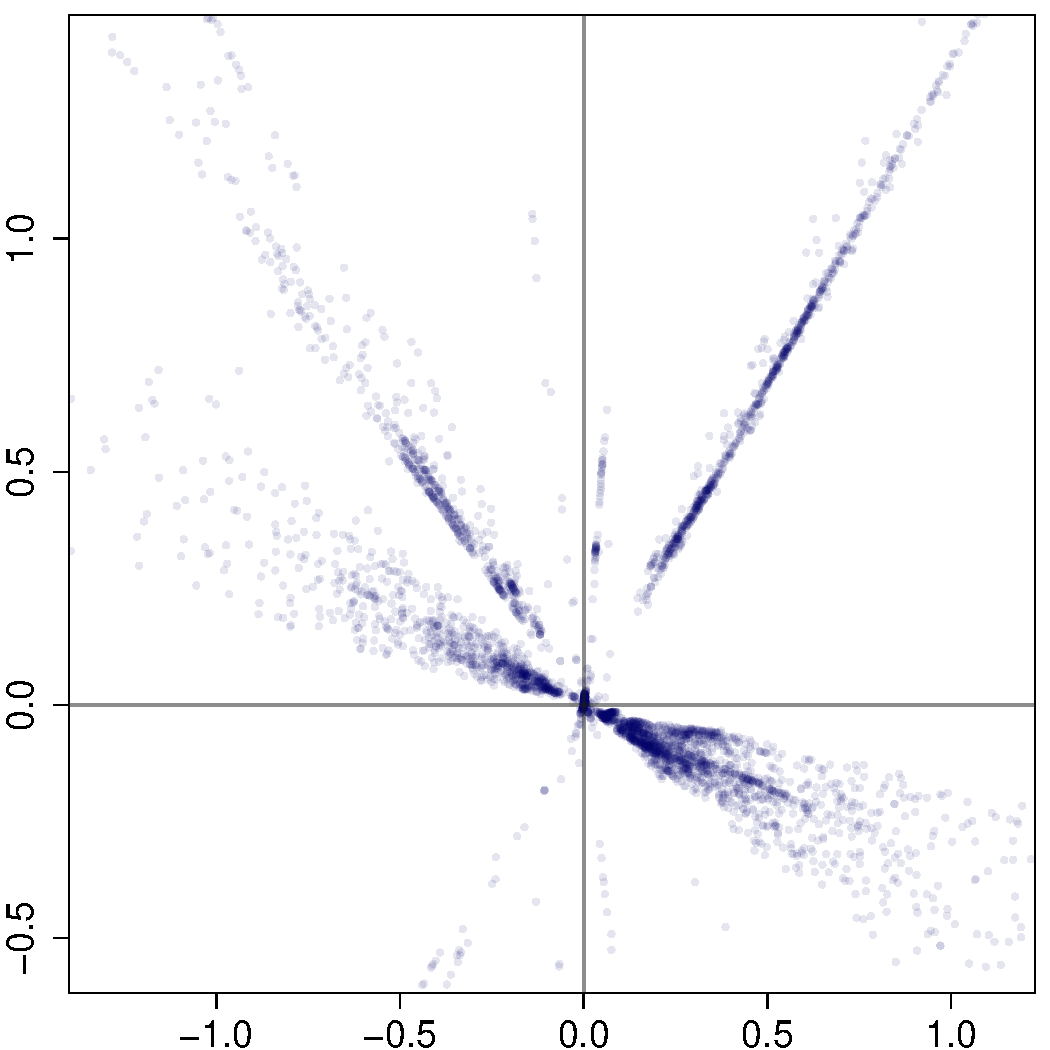
\includegraphics[width=1.6in]{svd/ie67}}
\subfloat[\footnotesize{SIGCOMM 2004}]{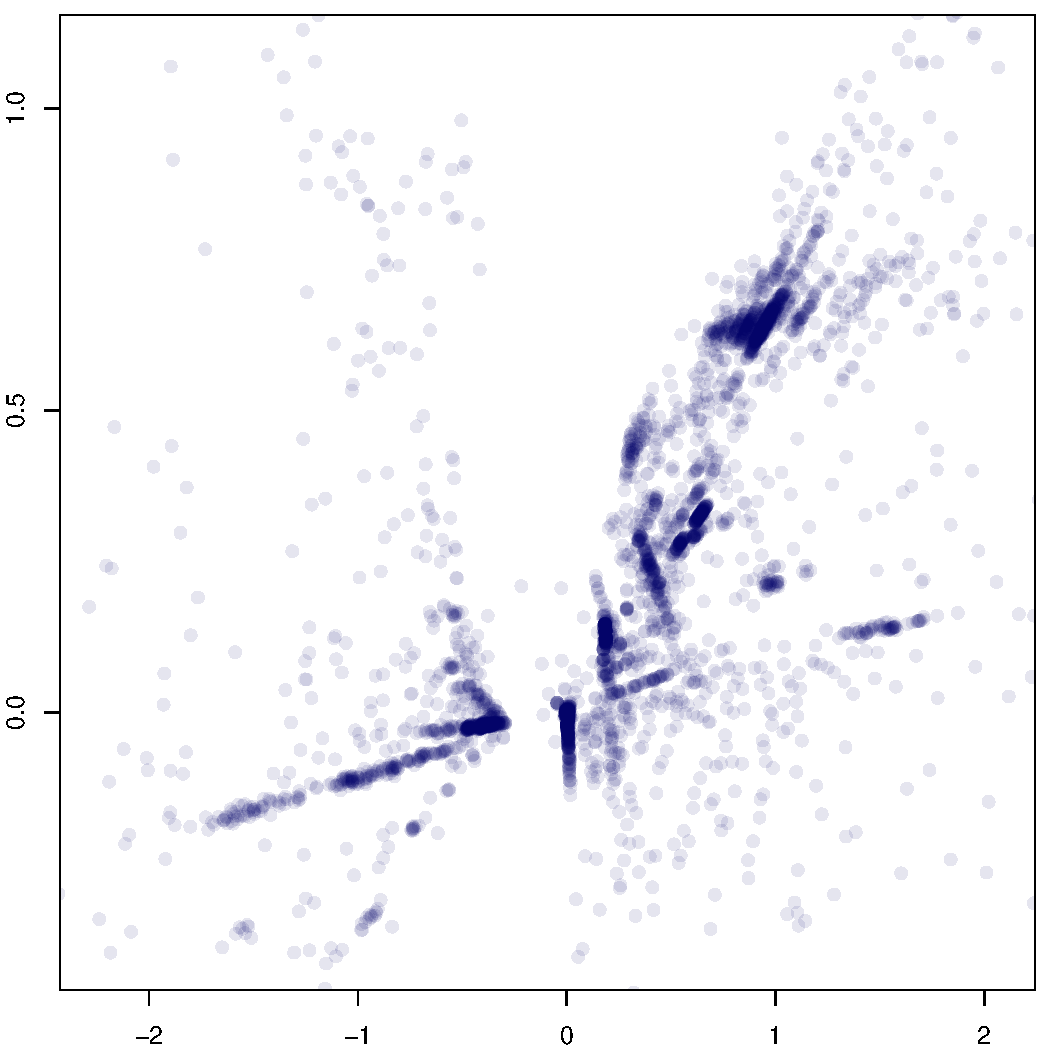
\includegraphics[width=1.6in]{svd/sc04}}
\subfloat[\footnotesize{UCSD}]{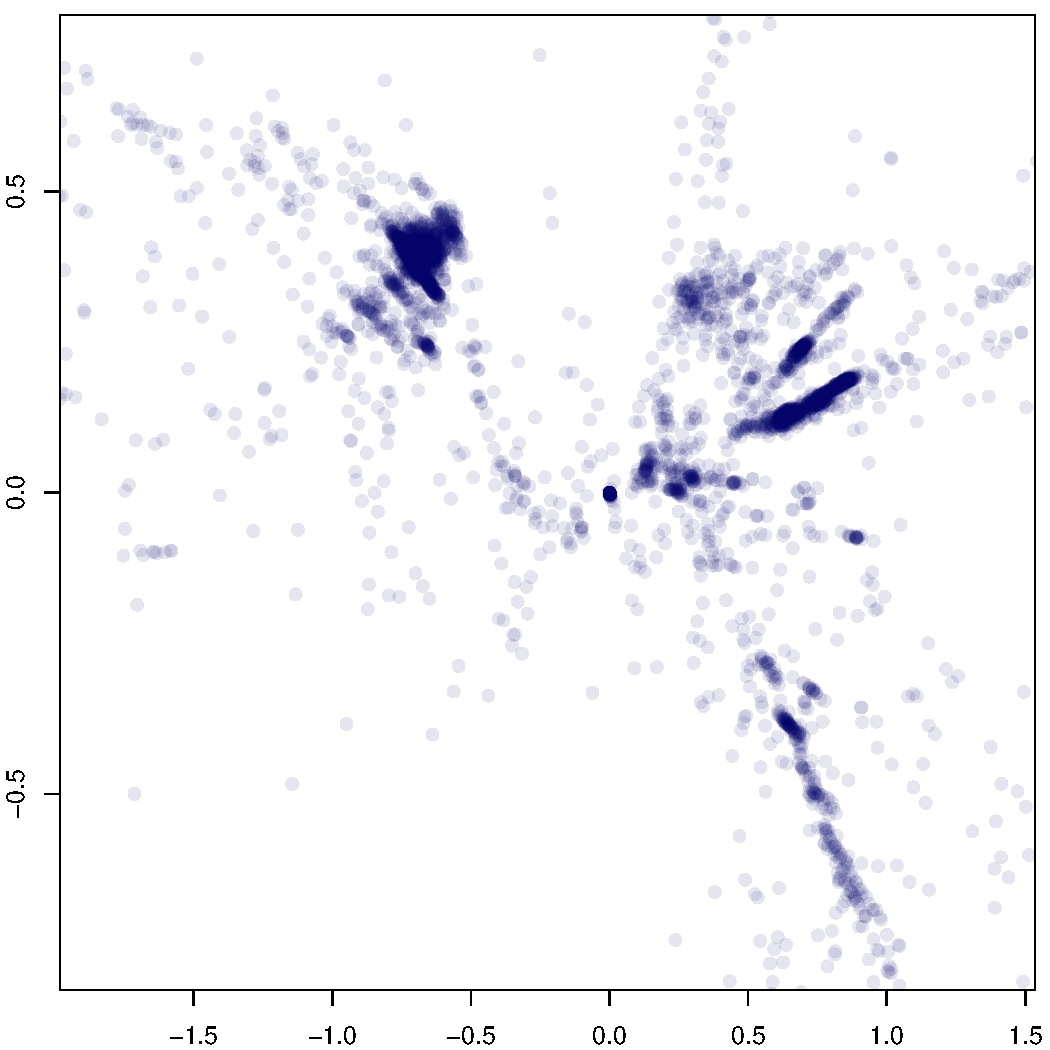
\includegraphics[width=1.6in]{svd/ucsd}}
\caption{SVD scatter plots for various traces.} 
\fig{svd}
\end{center}
\vspace{-0.85em}
\end{figure}

Clearly visible in \Figure{svd} is linear structure:
points are heavily concentrated on low-dimensional subspaces.
Because of the projection step of our process, points concentrated along a one-dimensional subspace appear as dark ``spots'' where many points have been plotted;
points concentrated along a two-dimensional subspace appear as lines;
points falling along subspaces of three or more dimensions appear as ``smears.''

\section{Methodology}\sec{methodology}

\section{Results}\sec{results}

\section{Discussion}\sec{discussion}

\section{Conclusions}\sec{conclusions}

\bibliography{IEEE,references}

\end{document}
